\documentclass[tikz, border=1cm]{standalone}

\usepackage{tikz}
\usetikzlibrary{calc}

\begin{document}
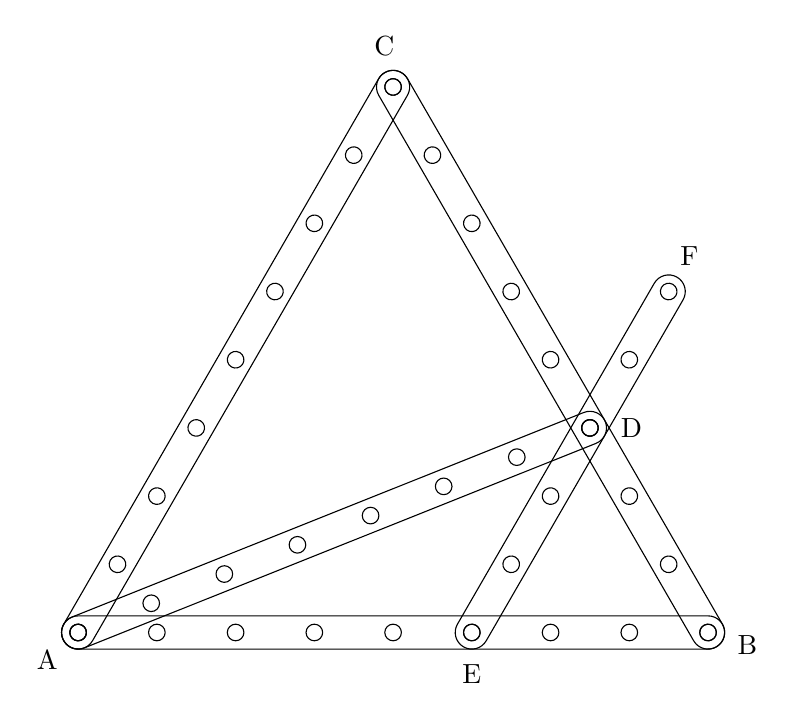
\begin{tikzpicture}

\begin{scope} %AB
 \draw (0,6pt) -- ++(8,0) arc(+90:-90:6pt) -- ++(-8,0) arc(270:90:6pt);
 \foreach \x in {0,1,...,8} 
 \draw (\x,0) circle (3pt);
 \path (0,0) ++(222:15pt) node{A};
 \path (5,0) ++(270:15pt) node{E};
\end{scope}

\begin{scope}[shift={(8,0)},rotate=120] %BC
 \draw (0,6pt) -- ++(8,0) arc(+90:-90:6pt) -- ++(-8,0) arc(270:90:6pt);
 \foreach \x in {0,1,...,8} 
 \draw (\x,0) circle (3pt);
 \path (0,0) ++(222:15pt) node{B};
 \path (3,0) ++(240:15pt) node{D};
  
 \begin{scope}[shift={(8,0)},rotate=120] %CA
  \draw (0,6pt) -- ++(8,0) arc(+90:-90:6pt) -- ++(-8,0) arc(270:90:6pt);
  \foreach \x in {0,1,...,8} 
  \draw (\x,0) circle (3pt);
  \path (0,0) ++(222:15pt) node{C};
 \end{scope}
  
\end{scope}

\begin{scope}[shift={(0,0)},rotate=21.7868] %AD
 \draw (0,6pt) -- ++(7,0) arc(+90:-90:6pt) -- ++(-7,0) arc(270:90:6pt);
 \foreach \x in {0,1,...,7} 
 \draw (\x,0) circle (3pt);
\end{scope}

\begin{scope}[shift={(5,0)},rotate=60] %EF
 \draw (0,6pt) -- ++(5,0) arc(+90:-90:6pt) -- ++(-5,0) arc(270:90:6pt);
 \foreach \x in {0,1,...,5} 
 \draw (\x,0) circle (3pt);
 \path (5,0) ++(0:15pt) node{F};
\end{scope}

\end{tikzpicture}
\end{document}
